\section{zesto-oracle.h File Reference}
\label{zesto-oracle_8h}\index{zesto-oracle.h@{zesto-oracle.h}}
{\tt \#include \char`\"{}zesto-cache.h\char`\"{}}\par


Include dependency graph for zesto-oracle.h:\nopagebreak
\begin{figure}[H]
\begin{center}
\leavevmode
\includegraphics[width=61pt]{zesto-oracle_8h__incl}
\end{center}
\end{figure}


This graph shows which files directly or indirectly include this file:\nopagebreak
\begin{figure}[H]
\begin{center}
\leavevmode
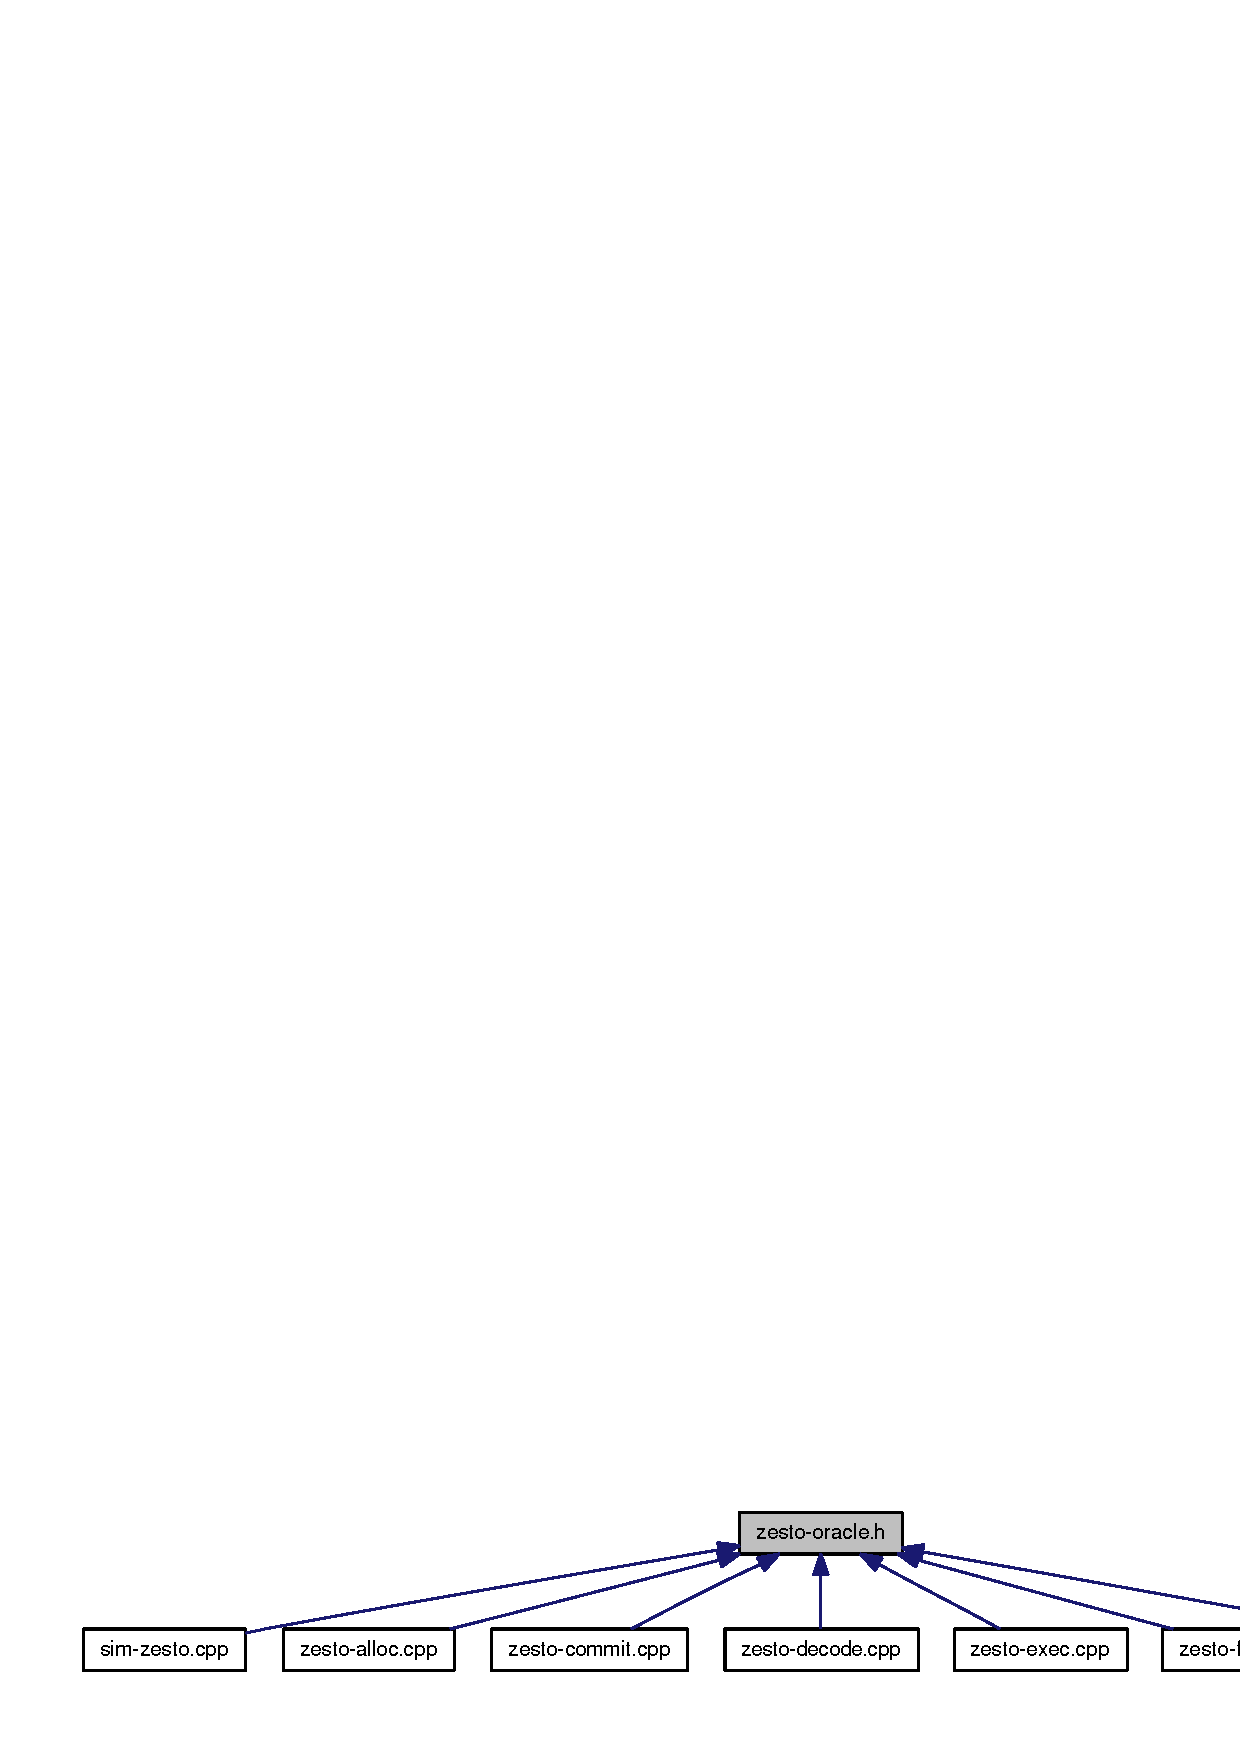
\includegraphics[width=376pt]{zesto-oracle_8h__dep__incl}
\end{center}
\end{figure}
\subsection*{Classes}
\begin{CompactItemize}
\item 
class {\bf core\_\-oracle\_\-t}
\item 
struct {\bf core\_\-oracle\_\-t::core\_\-oracle\_\-t::map\_\-node\_\-t}
\item 
struct {\bf core\_\-oracle\_\-t::core\_\-oracle\_\-t::spec\_\-mem\_\-t}
\item 
struct {\bf core\_\-oracle\_\-t::core\_\-oracle\_\-t::syscall\_\-mem\_\-req\_\-t}
\end{CompactItemize}
\subsection*{Defines}
\begin{CompactItemize}
\item 
\#define {\bf USE\_\-PIN\_\-TRACES}
\item 
\#define {\bf zesto\_\-fatal}(msg, retval)
\item 
\#define {\bf zesto\_\-assert}(cond, retval)
\item 
\#define {\bf MEM\_\-HASH\_\-SIZE}~32768
\item 
\#define {\bf MEM\_\-HASH\_\-MASK}~(MEM\_\-HASH\_\-SIZE-1)
\item 
\#define {\bf MD\_\-FETCH\_\-INST}(INST, MEM, PC, ID)~md\_\-fetch\_\-inst(\&INST, MEM, PC, ID)
\item 
\#define {\bf MD\_\-FETCH\_\-NEXT\_\-PC}(nextPC, ID)~md\_\-fetch\_\-next\_\-pc(\&nextPC,ID)
\end{CompactItemize}
\subsection*{Functions}
\begin{CompactItemize}
\item 
void {\bf md\_\-fetch\_\-inst} ({\bf md\_\-inst\_\-t} $\ast$inst, struct {\bf mem\_\-t} $\ast$mem, const {\bf md\_\-addr\_\-t} pc, unsigned int core\_\-id)
\item 
{\bf md\_\-addr\_\-t} {\bf md\_\-fetch\_\-next\_\-pc} ({\bf md\_\-addr\_\-t} $\ast$nextPC, unsigned int core\_\-id)
\end{CompactItemize}


\subsection{Define Documentation}
\index{zesto-oracle.h@{zesto-oracle.h}!MD\_\-FETCH\_\-INST@{MD\_\-FETCH\_\-INST}}
\index{MD\_\-FETCH\_\-INST@{MD\_\-FETCH\_\-INST}!zesto-oracle.h@{zesto-oracle.h}}
\subsubsection[{MD\_\-FETCH\_\-INST}]{\setlength{\rightskip}{0pt plus 5cm}\#define MD\_\-FETCH\_\-INST(INST, \/  MEM, \/  PC, \/  ID)~md\_\-fetch\_\-inst(\&INST, MEM, PC, ID)}\label{zesto-oracle_8h_465a782fc5c7f5e58a637011cd6c26ed}




Definition at line 303 of file zesto-oracle.h.

Referenced by core\_\-oracle\_\-t::exec(), and sim\_\-fastfwd().\index{zesto-oracle.h@{zesto-oracle.h}!MD\_\-FETCH\_\-NEXT\_\-PC@{MD\_\-FETCH\_\-NEXT\_\-PC}}
\index{MD\_\-FETCH\_\-NEXT\_\-PC@{MD\_\-FETCH\_\-NEXT\_\-PC}!zesto-oracle.h@{zesto-oracle.h}}
\subsubsection[{MD\_\-FETCH\_\-NEXT\_\-PC}]{\setlength{\rightskip}{0pt plus 5cm}\#define MD\_\-FETCH\_\-NEXT\_\-PC(nextPC, \/  ID)~md\_\-fetch\_\-next\_\-pc(\&nextPC,ID)}\label{zesto-oracle_8h_486f7c7db21691d4d34a7818717e98b8}




Definition at line 305 of file zesto-oracle.h.

Referenced by emergency\_\-recovery(), core\_\-oracle\_\-t::exec(), sim\_\-fastfwd(), and sim\_\-main().\index{zesto-oracle.h@{zesto-oracle.h}!MEM\_\-HASH\_\-MASK@{MEM\_\-HASH\_\-MASK}}
\index{MEM\_\-HASH\_\-MASK@{MEM\_\-HASH\_\-MASK}!zesto-oracle.h@{zesto-oracle.h}}
\subsubsection[{MEM\_\-HASH\_\-MASK}]{\setlength{\rightskip}{0pt plus 5cm}\#define MEM\_\-HASH\_\-MASK~(MEM\_\-HASH\_\-SIZE-1)}\label{zesto-oracle_8h_d2111e2165e4a519d36c3f3af50d557e}




Definition at line 190 of file zesto-oracle.h.

Referenced by core\_\-oracle\_\-t::commit\_\-write\_\-byte(), core\_\-oracle\_\-t::spec\_\-read\_\-byte(), core\_\-oracle\_\-t::spec\_\-write\_\-byte(), and core\_\-oracle\_\-t::squash\_\-write\_\-byte().\index{zesto-oracle.h@{zesto-oracle.h}!MEM\_\-HASH\_\-SIZE@{MEM\_\-HASH\_\-SIZE}}
\index{MEM\_\-HASH\_\-SIZE@{MEM\_\-HASH\_\-SIZE}!zesto-oracle.h@{zesto-oracle.h}}
\subsubsection[{MEM\_\-HASH\_\-SIZE}]{\setlength{\rightskip}{0pt plus 5cm}\#define MEM\_\-HASH\_\-SIZE~32768}\label{zesto-oracle_8h_9f1b1e541085cdd8c4585b1d583e87ed}




Definition at line 189 of file zesto-oracle.h.\index{zesto-oracle.h@{zesto-oracle.h}!USE\_\-PIN\_\-TRACES@{USE\_\-PIN\_\-TRACES}}
\index{USE\_\-PIN\_\-TRACES@{USE\_\-PIN\_\-TRACES}!zesto-oracle.h@{zesto-oracle.h}}
\subsubsection[{USE\_\-PIN\_\-TRACES}]{\setlength{\rightskip}{0pt plus 5cm}\#define USE\_\-PIN\_\-TRACES}\label{zesto-oracle_8h_3ad9043475baaed1a4a792d3b563c60d}




Definition at line 140 of file zesto-oracle.h.\index{zesto-oracle.h@{zesto-oracle.h}!zesto\_\-assert@{zesto\_\-assert}}
\index{zesto\_\-assert@{zesto\_\-assert}!zesto-oracle.h@{zesto-oracle.h}}
\subsubsection[{zesto\_\-assert}]{\setlength{\rightskip}{0pt plus 5cm}\#define zesto\_\-assert(cond, \/  retval)}\label{zesto-oracle_8h_4f942292a4c30024a9b7fe4f9b1820a4}


\textbf{Value:}

\begin{Code}\begin{verbatim}{ \
  if(!(cond)) { \
    core->oracle->hosed = TRUE; \
    fprintf(stderr,"assertion failed (%s,%d:thread %d): ",__FILE__,__LINE__,core->current_thread->id); \
    fprintf(stderr,"%s\n",#cond); \
    return (retval); \
  } \
}
\end{verbatim}
\end{Code}


Definition at line 169 of file zesto-oracle.h.

Referenced by core\_\-exec\_\-STM\_\-t::ALU\_\-exec(), core\_\-exec\_\-DPM\_\-t::ALU\_\-exec(), core\_\-decode\_\-STM\_\-t::check\_\-flush(), core\_\-decode\_\-DPM\_\-t::check\_\-flush(), core\_\-exec\_\-STM\_\-t::check\_\-load\_\-issue\_\-conditions(), core\_\-exec\_\-DPM\_\-t::check\_\-load\_\-issue\_\-conditions(), core\_\-oracle\_\-t::commit\_\-uop(), core\_\-exec\_\-STM\_\-t::DL1\_\-callback(), core\_\-exec\_\-STM\_\-t::DTLB\_\-callback(), core\_\-exec\_\-DPM\_\-t::DTLB\_\-callback(), core\_\-exec\_\-STM\_\-t::insert\_\-ready\_\-uop(), core\_\-exec\_\-DPM\_\-t::insert\_\-ready\_\-uop(), core\_\-exec\_\-STM\_\-t::LDQ\_\-squash(), core\_\-exec\_\-DPM\_\-t::LDQ\_\-squash(), core\_\-exec\_\-STM\_\-t::LDST\_\-exec(), core\_\-exec\_\-DPM\_\-t::LDST\_\-exec(), core\_\-exec\_\-DPM\_\-t::load\_\-miss\_\-reschedule(), core\_\-exec\_\-STM\_\-t::load\_\-writeback(), core\_\-exec\_\-DPM\_\-t::load\_\-writeback(), core\_\-fetch\_\-DPM\_\-t::Mop\_\-consume(), core\_\-fetch\_\-STM\_\-t::Mop\_\-peek(), core\_\-oracle\_\-t::pipe\_\-flush(), core\_\-decode\_\-STM\_\-t::recover(), core\_\-decode\_\-DPM\_\-t::recover(), core\_\-commit\_\-STM\_\-t::recover(), core\_\-commit\_\-DPM\_\-t::recover(), core\_\-alloc\_\-DPM\_\-t::recover(), core\_\-exec\_\-STM\_\-t::recover\_\-check\_\-assertions(), core\_\-exec\_\-DPM\_\-t::recover\_\-check\_\-assertions(), core\_\-decode\_\-DPM\_\-t::recover\_\-decode\_\-pipe(), core\_\-exec\_\-STM\_\-t::RS\_\-deallocate(), core\_\-exec\_\-DPM\_\-t::RS\_\-deallocate(), core\_\-alloc\_\-STM\_\-t::RS\_\-deallocate(), core\_\-alloc\_\-DPM\_\-t::RS\_\-deallocate(), core\_\-exec\_\-STM\_\-t::RS\_\-schedule(), core\_\-exec\_\-DPM\_\-t::RS\_\-schedule(), core\_\-exec\_\-DPM\_\-t::snatch\_\-back(), core\_\-fetch\_\-STM\_\-t::step(), core\_\-fetch\_\-DPM\_\-t::step(), core\_\-decode\_\-STM\_\-t::step(), core\_\-decode\_\-DPM\_\-t::step(), core\_\-commit\_\-STM\_\-t::step(), core\_\-commit\_\-DPM\_\-t::step(), core\_\-alloc\_\-STM\_\-t::step(), core\_\-alloc\_\-DPM\_\-t::step(), core\_\-exec\_\-STM\_\-t::store\_\-dl1\_\-callback(), core\_\-exec\_\-DPM\_\-t::store\_\-dl1\_\-callback(), core\_\-exec\_\-DPM\_\-t::store\_\-dl1\_\-split\_\-callback(), core\_\-exec\_\-STM\_\-t::store\_\-dtlb\_\-callback(), core\_\-exec\_\-DPM\_\-t::store\_\-dtlb\_\-callback(), core\_\-exec\_\-DPM\_\-t::store\_\-translated\_\-callback(), core\_\-exec\_\-DPM\_\-t::STQ\_\-deallocate\_\-senior(), core\_\-exec\_\-STM\_\-t::STQ\_\-insert\_\-std(), core\_\-exec\_\-DPM\_\-t::STQ\_\-insert\_\-std(), core\_\-exec\_\-STM\_\-t::STQ\_\-squash\_\-sta(), core\_\-exec\_\-DPM\_\-t::STQ\_\-squash\_\-sta(), core\_\-exec\_\-STM\_\-t::STQ\_\-squash\_\-std(), core\_\-exec\_\-DPM\_\-t::STQ\_\-squash\_\-std(), core\_\-decode\_\-STM\_\-t::uop\_\-consume(), and core\_\-decode\_\-STM\_\-t::uop\_\-peek().\index{zesto-oracle.h@{zesto-oracle.h}!zesto\_\-fatal@{zesto\_\-fatal}}
\index{zesto\_\-fatal@{zesto\_\-fatal}!zesto-oracle.h@{zesto-oracle.h}}
\subsubsection[{zesto\_\-fatal}]{\setlength{\rightskip}{0pt plus 5cm}\#define zesto\_\-fatal(msg, \/  retval)}\label{zesto-oracle_8h_a62f33e5d3102234e8f957f4722f5f51}


\textbf{Value:}

\begin{Code}\begin{verbatim}{ \
  core->oracle->hosed = TRUE; \
  fprintf(stderr,"fatal (%s,%d:thread %d): ",__FILE__,__LINE__,core->current_thread->id); \
  fprintf(stderr,"%s\n",msg); \
  return (retval); \
}
\end{verbatim}
\end{Code}


Definition at line 158 of file zesto-oracle.h.

\subsection{Function Documentation}
\index{zesto-oracle.h@{zesto-oracle.h}!md\_\-fetch\_\-inst@{md\_\-fetch\_\-inst}}
\index{md\_\-fetch\_\-inst@{md\_\-fetch\_\-inst}!zesto-oracle.h@{zesto-oracle.h}}
\subsubsection[{md\_\-fetch\_\-inst}]{\setlength{\rightskip}{0pt plus 5cm}void md\_\-fetch\_\-inst ({\bf md\_\-inst\_\-t} $\ast$ {\em inst}, \/  struct {\bf mem\_\-t} $\ast$ {\em mem}, \/  const {\bf md\_\-addr\_\-t} {\em pc}, \/  unsigned int {\em core\_\-id})}\label{zesto-oracle_8h_c9b36de1d166dbea41697884bd42aa7e}




Definition at line 2230 of file zesto-oracle.cpp.

References md\_\-inst\_\-t::code, cores, mem\_\-ops::ld\_\-dequeued, mem\_\-ops::ld\_\-size, md\_\-inst\_\-t::mem\_\-ops, mem\_\-ops::mem\_\-paddr\_\-ld, mem\_\-ops::mem\_\-paddr\_\-str, MEM\_\-RD, mem\_\-ops::mem\_\-vaddr\_\-ld, mem\_\-ops::mem\_\-vaddr\_\-str, MEM\_\-WR, mem\_\-ops::memops, md\_\-inst\_\-t::paddr, md\_\-inst\_\-t::qemu\_\-len, sim\_\-exit\_\-buf, store\_\-nextPC, mem\_\-ops::str\_\-dequeued, mem\_\-ops::str\_\-size, use\_\-stored\_\-nextPC, and md\_\-inst\_\-t::vaddr.\index{zesto-oracle.h@{zesto-oracle.h}!md\_\-fetch\_\-next\_\-pc@{md\_\-fetch\_\-next\_\-pc}}
\index{md\_\-fetch\_\-next\_\-pc@{md\_\-fetch\_\-next\_\-pc}!zesto-oracle.h@{zesto-oracle.h}}
\subsubsection[{md\_\-fetch\_\-next\_\-pc}]{\setlength{\rightskip}{0pt plus 5cm}{\bf md\_\-addr\_\-t} md\_\-fetch\_\-next\_\-pc ({\bf md\_\-addr\_\-t} $\ast$ {\em nextPC}, \/  unsigned int {\em core\_\-id})}\label{zesto-oracle_8h_4603dc5f3e60fbfcd30343123777d18c}




Definition at line 2429 of file zesto-oracle.cpp.

References cores, core\_\-t::current\_\-thread, core\_\-t::fetch, core\_\-fetch\_\-t::PC, thread\_\-t::pin\_\-trace, thread\_\-t::regs, regs\_\-t::regs\_\-NPC, regs\_\-t::regs\_\-PC, store\_\-nextPC, and use\_\-stored\_\-nextPC.

Referenced by core\_\-oracle\_\-t::pipe\_\-flush().

Here is the caller graph for this function:\nopagebreak
\begin{figure}[H]
\begin{center}
\leavevmode
\includegraphics[width=246pt]{zesto-oracle_8h_4603dc5f3e60fbfcd30343123777d18c_icgraph}
\end{center}
\end{figure}
